\chapter{Joint Decisions}
\label{ch:jointtrips}
% ##################################################################################################################

\hfill \textbf{Author:} Thibaut Dubernet

\begin{center} 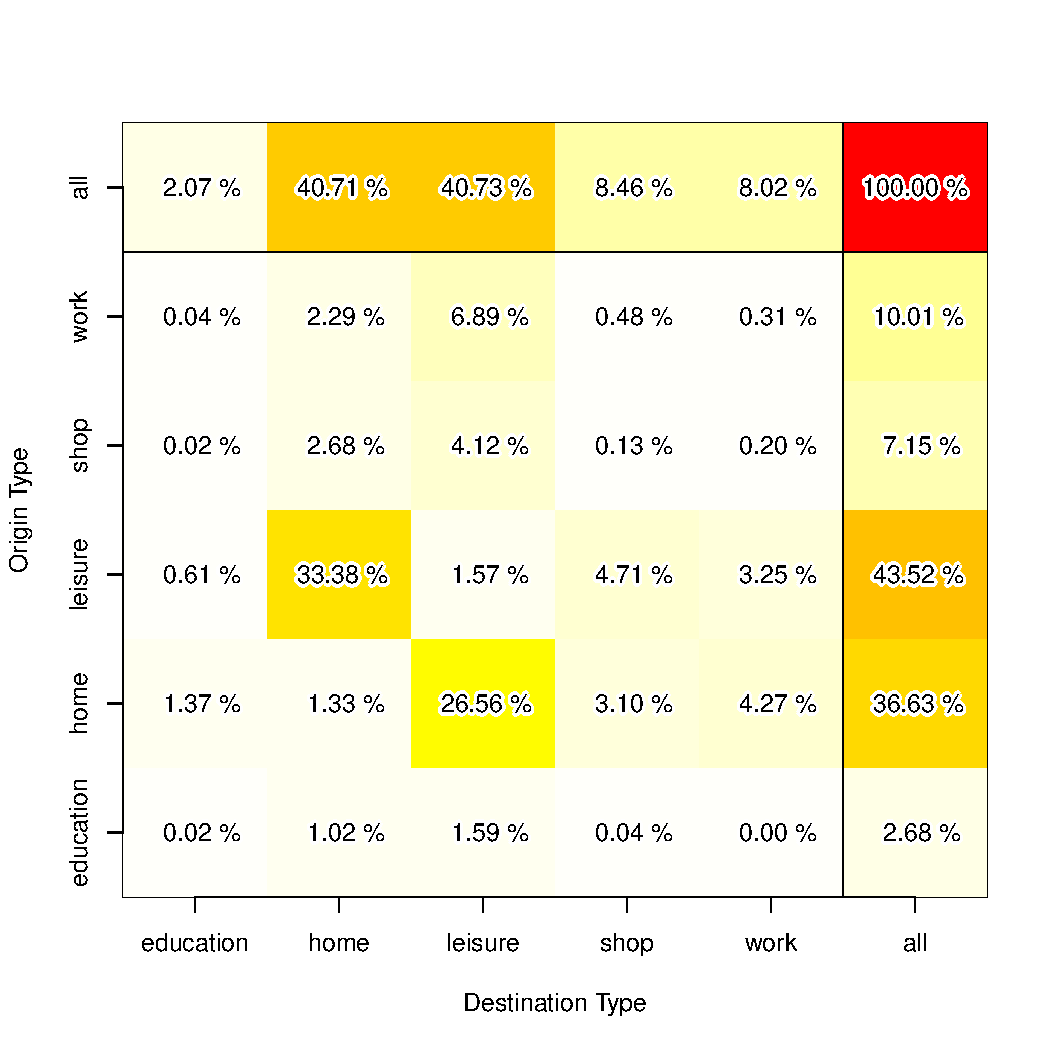
\includegraphics[width=0.4\textwidth, angle=0]{extending/figures/Jointtrips/passenger-per-type-ju3-asShareOfPassengerTrips} \end{center}

\createStandardInformation{todo}{todo}{todo}{todo}

% ##################################################################################################################
{ % scope for our commands: do not pollute our little friends

% ##################################################################################################################

\newcommand\authoranddate{\citet}
\renewcommand\cite\citep

\newcommand\eg{\emph{e.g.}\xspace}
\newcommand\ie{\emph{i.e.}\xspace}
\newcommand\pudptw{Pick-Up and Delivery Problem With Time Windows\xspace}
\newcommand\structeqmodel{structural equation model\xspace}
\newcommand\ga{genetic algorithm\xspace}
\newcommand\gas{genetic algorithms\xspace}
\newcommand\Gas{Genetic algorithms\xspace}
\newcommand\mz{National Travel Survey\xspace}
\newcommand\matsim{MATSim\xspace}

% to hide todos in this section
\renewcommand\todo[1]{}

% Figures crap
\newcommand\insfig[2]{%
	\insfigwidth{#1}{#2}{.8\textwidth}
}
\newcommand\insfigwidth[3]{%
\createfigure{#1}{#1}{}{%
		\includegraphics[width=#3]{extending/figures/Jointtrips/#2}%
		}{}%
}

\newcommand\inssubfigwidth[3]{%
\createsubfigure{#2}{%
		\includegraphics[width=#1]{extending/figures/Jointtrips/#3}%
		}{}{\quad}%
}
\newcommand\inssubfig[2]{%
\inssubfigwidth{.46\textwidth}{#1}{#2}%
}
\newcommand\insfigwithsubfigs[2]{%
\createfigure{#1}{#1}{}{%
		#2%
		}{}%
}

% ##################################################################################################################
This chapter describes the extension of \matsim to consider what we name \emph{joint decisions}.
\cref{sec:td:intro} explains what we name joint decision, and gives an overview of why such processes
are important in transportation.
\cref{sec:td:algo} then presents concepts to model this behavior,
presents a generalization of the \matsim algorithm to search for solutions to what
we call the \emph{joint planning problem},
and gives technical insights on how this implementation could be achieved,
given the \matsim software architecture.

% ##################################################################################################################
\section{Joint Decisions and Transport Systems\label{sec:td:intro}}
\subsection{Motivation}
\todo{Shorten this A LOT!!!!}

In recent years, there has been a growing interest in the social dimension of travel,
and how travel decisions are influenced not only by the global state of the transportation system,
but also by joint decisions and interactions with social contacts.

A very active field of research is the study and modeling of intrahousehold interactions
and joint decision making, % \cite{TimmermansZhang_TransResB_2009},
often using the classical random utility framework extended to group decision making.
%
Examples of household scheduling models include
\authoranddate{ZhangEtAl_TransResB_2005},
%
\authoranddate{ZhangJEtAl_TRR_2007},
%
% For instance,
\authoranddate{KatoMatsumoto_TransResB_2009},
%
\authoranddate{BradleyVovsha_Transportation_2005},
%
\authoranddate{GliebeKoppelman_Transportation_2005},
%
\authoranddate{GliebeKoppelman_Transportation_2002},
%
\authoranddate{HoCAndMulley_Transportation_2013},
%
or
\authoranddate{VovshaGupta_Transportation_2013}.
%
Most of those models
are specific to given household structures;
in particular, separate models need to be estimated for different household sizes.

%Household level decision processes have also been modeled with approaches which significantly differ
%from the classical random utility framework.
%%
%\authoranddate{GolobMcNally_TransResB_1997}
%propose a \structeqmodel,
%which predicts time allocation and trip chaining based on the sociodemographics of a household.
%\authoranddate{Golob_TransResB_2000}
%also used a \structeqmodel to model the dependency of time allocations
%of the two heads (man and woman) of a household.
%%

%
Another class of approaches,
more oriented toward multiagent simulation than analysis,
is the use of optimization algorithms to generate households plans.
They handle the household scheduling problem by transforming it into a deterministic utility maximization problem.
Contrary to the previously presented approaches,
those alternatives do not lead to the estimation of a model against data.
%However, the estimation of the utility function is usually not part of those approaches.
%
Examples of approaches rooted in operations research include
\authoranddate{Recker_TRR_1995},
for which \authoranddate{ChowRecker_TranResB_2012}
designed a calibration method,
or \authoranddate{GanRecker_TransResB_2008}.
%
Another attempt to generate plans for households uses a \ga,
building on a previous \ga for individual plan generation
\cite{CharyparNagel_Transportation_2005,MeisterEtAl_Transportation_2005},
using a joint utility.
%
Finally, \authoranddate{LiaoFEtAl_Transportation_2013} formulate the problem of creating
schedules for two persons traveling together as finding the shortest path
in a ``supernetwork'',
but note that their model is specific to the two person problem,
and that extension to larger numbers of agents may prove to be computationally expensive.
%
%Finally, Fang \emph{et al.} optimize location and time of joint activities, constrained to time windows in pre-determined individual plans, using a multi-objective \ga \cite{Fang2011}.
All those approaches remained experimental,
and were not integrated into multiagent simulation tools.

Another class of methods aiming at multiagent simulations
is constituted rule based systems,
which use heuristic rules to construct household plans,
%
such as
\authoranddate{MillerEtAl_Transportation_2005}
or
%
\authoranddate{ArentzeTimmermans_TransResB_2009}.

Other authors have investigated the role of more general social networks on travel.
One of the main incentives to conduct such studies comes from the continuous increase of the share of
trips which are performed for leisure purpose
\cite{SchlichEtAl_TransportRev_2004,Axhausen_DonaghyEtAl_2005}.
This fact represents a challenge for travel behavior modeling,
as those trips are much more difficult to forecast than commuting trips:
they are performed more sporadically, and data about those trips is much more difficult to collect
--- in particular concerning attributes of locations and events,
which are needed to make models that do not only consist of random noise.
Understanding better how destination choice for leisure trip is made is therefore essential to improve
the accuracy of those forecasts.

Various studies have been conducted with the idea that an important factor in leisure trip destination
choice, or activity duration choice, is the ability to meet social contacts.
Examples of empirical work include \authoranddate{CarrascoJAHabib_IATBR_2009}; \authoranddate{HabibCarrascoJA_TRR_2011} or \authoranddate{MooreJEtAl_Transportation_2013}.
All those studies show a substantial influence of social contacts on the spatial and temporal
distribution of activities.
%
%Based on an analysis of social network involvement and role, \authoranddate{DeutschGoulias_Transportation_2013}
%advocate considering the \emph{role} individuals play in different social networks.
%Using latent class cluster analysis models to analyse the role of individuals in
%the various social networks they are involved in,
%they find that ``the decision-making role of an individual can differ vastly across different
%social engagement types''.
%
\authoranddate{Frei_PhDThesis_2012} demonstrated in a simulation experiment how considering social interactions
in leisure location choice can help increase the accuracy of predicted leisure trip distance distribution.

Another field of empirical research studies the spatial characteristics of social networks.
For instance, \authoranddate{CarrascoJAEtAl_TRR_2008} studied the relationship between individual's socioeconomic
characteristics and the spatial distribution of their social contacts.
This kind of empirical work allows to specify and estimate models able to generate synthetic social networks,
given sociodemographic attributes and home location.
An example of such a model, based on the results of a survey in Switzerland,
can be found in \authoranddate{ArentzeEtAl_TRB_2012}.
This kind of model is essential if one wants to include social network interactions
in microsimulation model.

This integration of social networks in multiagent simulation frameworks has already
been attempted by other authors.
Due to their disaggregated description of the world,
such models are particularly well suited to the representation of complex social topologies.
\authoranddate{HanQEtAl_TransResPartA_2011} present experiments of using social networks
to guide activity location choice set formation in the FEATHERS multiagent simulation framework.
Using a simple scenario with 6 agents forming a \emph{clique},
%(a network where all agents have social ties with all other agents),
they consider the influence of various processes like
information exchange and adaptation to the behavior of social contacts to increase the probability
of an encounter.
They do not, however, represent \emph{joint decisions}, such as the scheduling of a joint activity.
The same kind of processes have been investigated by \authoranddate{Hackney_PhDThesis_2009},
using more complex network topologies,
within the \matsim framework, used in this paper.
\authoranddate{RonaldEtAl_TransResB_2012}
and \authoranddate{MaEtAl_TRR_2011,MaEtAl_IATBR_2012}
present agent based systems which do integrate
joint decision making mechanisms,
based on rule based simulations of a bargaining processes.
They are not yet integrated into
any operational mobility simulation platform.

Those remarks point the need\todo{other word\ldots too strong}
to include explicit coordination in multiagent simulation platforms.

\subsection{The Joint Planning Problem}
%---------------------------------------------------------------------------

\todo{define the ``problem''\ldots}

We present here a simulation framework able to represent \emph{joint decisions},
that is, behavior requiring \emph{explicit} coordination between individuals
--- such as shared rides, social activities or intra-household task allocation.
The basic idea is that social contacts will take such a joint decision if it results
in an improvement in the satisfaction of all participants.
The modeling of the interaction of individuals with possibly conflicting objectives
has been the subject of game theory for decades, making this theoretical framework
particularly well suited for the problem at hand.

\todo{make terminology consistent, between individual, player and agent}
A game theoretic view of transportation systems has indeed been popular
since the seminal work of
\citeauthor{Wardrop_PICE_1952}
\cite{Wardrop_PICE_1952}.
The essential idea behind it is to see the transportation system as
a set of shared resources (road space, public transport vehicle seats\ldots),
for which individuals compete, individuals in the population trying to maximize
their own satisfaction, given the resources left available by others.
Game theory studies \emph{solution concepts} for such strategic interactions.
A game theoretic solution concept is a definition of which states are
\emph{equilibria}, that is,
%considered
\emph{stable} under assumption of rationality
--- a state being considered stable if no agent/player has an incentive
to change its behavior.
%
The static, trip-based approach of
\citeauthor{Wardrop_PICE_1952}
has been refined and extended with time.
In particular, the equilibrium idea can be pretty naturally transfered to
the \emph{activity based} framework:
individuals do not just try to optimize their trips, 
but their whole day.
\todo{formulate better, but remain short}%
This is in particular the approach of the \matsim software framework
\cite{Axhausen_SSRL_2006,NagelFloetteroed_IATBR_2009}.

Most solution concepts in transportation are akin to the Nash equilibrium:
a state where no individual can improve its satisfaction
by \emph{unilaterally} changing its behavior.
%
This kind of solution concept does not allow to represent joint decisions.
This can be illustrated by a classical game, called the \emph{House Allocation Problem}
\cite{SchummerVohra_NisanEtAl_2007}.
This game consists of $n$ players and $n$ houses. Moreover, each player has its individual
ordering of the houses, from the most preferred to the least preferred,
and players prefer being allocated alone to any house rather than in the
same house as somebody else.
The strategy of a player is the house it chooses to live in.

An interesting feature of this game is that any one-to-one allocation of players to houses is a
Nash Equilibrium: no player can improve its payoff by \emph{unilaterally} changing its strategy,
as it would require choosing an occupied house.
This result however contradicts basic intuition about the stability of such an allocation.
In this particular case, a more realistic solution concept is the \emph{Absence of Blocking Coalition}:
given a one-to-one allocation of houses to players, a blocking coalition is a set of players
which could all be better off by re-allocating their houses among themselves.
%
It is to be noted that both solution concepts correspond to rational agents, \ie agents having
a preference ordering over outcomes.
The only difference lies in the degree
of communication which is allowed.

In the activity-based framework, this solution concept naturally becomes what we phrase
the \emph{Absence of Improving Coalition} solution concept.
An improving coalition for a given allocation of daily plans
is a set of social contacts that can all be better off by \emph{simultaneously} changing
their daily plan
--- for instance by switching from separate dinners at home to a joint dinner at a restaurant.
The simulation of joint decision consists in the search of an allocation of daily plans
without such coalitions.


% ##################################################################################################################
\section{An Solution Algorithm for the Joint Planning Problem: a Generalization of the MATSim Process\label{sec:td:algo}}
\subsection{Algorithm}
%---------------------------------------------------------------------------

Given this theoretical framework, one needs to design and implement an
algorithm to search for allocations of daily plans to individuals, that
satisfy this solution concept.
This implementation consists of two
groups of components:

\begin{enumerate}
\item
  A \emph{Controller} that implements the extension of the MATSim
  co-evolutionary algorithm, outlined hereafter. It is implemented in a
  modular fashion, to be easily adapted to the specific need of
  different simulation scenarios
\item
  Specific implementations of the modular components,
  namely replanning strategies and scoring functions,
  to allow explore the set of possible \emph{joint plans},
  and represent possible preferences specific to joint decisions.
\end{enumerate}

\paragraph{Controller}

The MATSim framework provides a \emph{Controller} to build and configure
co-evolutionary algorithms, where agents each optimize their plan given
the (evolving) state of the transport system.

Unfortunately, this approach makes choices of agents independent ---
which of course goes against the simulation of \emph{joint decisions}.
To be able to implement an algorithm searching for states without
blocking coalitions, one needs a way to represent the influence of
explicit coordination on the utility of a daily plan. This is solved by
including \emph{joint plans} constraints. A joint plan is a set of
individual plans executed simultaneously. Different copies of the same
individual plan can be part of different joint plans --- for instance an
agent might go to a given restaurant alone, with members of its
household or with a group of friends. The score of the different copies
will take into account the influence of the joint plan to which it
pertains. Those joint plan constraints are included using heuristic
rules, applied after mutation operators are applied, and are classified
as strong or weak constraints --- weak constraints are considered when
selecting plans for execution, but are allowed to be broken when merely
selecting plans for mutation. They are then part of the evolution
process. In the current application, the heuristic rules consist in
joining newly created plans with joint trips (strong) or with leisure
activities at the same location at the same time (weak).

To allow handling joint plans, replanning needs to be performed for
groups of agents. This is straightforward for households: all agents of
a same household are always handled as a single group. For more general
social networks, agents are handled with all agents with whom they have
a joint plan, plus some social contacts with whom new joint plans can be
created.
%Details are presented in the ``Implementation'' section.

For each group, two actions are then possible. For most groups, an
allocation of existing plans, fulfilling the joint plans constraints, is
selected for execution. Based on plan scores, randomized by adding an
extreme value distributed error term, an allocation without improving
coalitions is searched for by an algorithm inspired by the ``Top Trading
Cycle'' algorithm used for the House Allocation Problem
\cite{SchummerVohra_NisanEtAl_2007}.

For the other groups, a plan allocation is selected and copied. The
copied plans then undertake mutation, to make the agents explore new
alternative joint plans. What kind of mutation is performed determines
which alternative plans will be tried out by the agent.
%The modules
%currently implemented are presented in the ``Implementation'' section.

Agents have a limited memory size, keeping by default at most 3 plans per joint
plan composition, and 10 plans in total. If this limit is exceeded, one
should keep the plans which have the highest probability to create
improving coalitions, that is, to be preferred to the other plans in the
agent's memory. To this end, a lexicographic ordering is used: the
process removes the joint plan which maximizes the number of individual
plans which are the worst of the agents' memories. If several joint
plans have the same number of worst plans, the process chooses among
them the joint plan which maximizes the number of second worst plans,
and so on until the ``worst'' joint plan is unique. When the overall
maximum number of plans in the memory of an agent is reached, the worst
individual plan for this agent is removed along with plans of other
agents of the same joint plan. Each agents keeps at least one plan not
part of a joint plan, as there may otherwise not be any state without
blocking coalitions. Agents are parsed in random order, to avoid the
emergence of ``dictators'' over iterations, whose worst plan would
always be removed, even if it is the only ``bad'' plan of a joint plan.

Though those selection operators seem to be in accordance with the
chosen solution concept, it is difficult, if not impossible, to prove
that the process will actually converge towards the state searched. As
noted by \authoranddate{FiciciEtAl_ITEC_2005}, when they perform a theoretical
analysis of different selection methods in a co-evolutionary context,
``Co-evolutionary dynamics are \emph{notoriously complex}. To focus on
our attention on selection dynamics, we will use a simple evolutionary
game-theoretic framework to eliminate \emph{confounding factors} such as
those related to genetic variation, noisy evaluation, and finite
population size''. Those ``confounding factors'' can however not be
eliminated from an actual implementation of a co-evolutionary algorithm,
and rigorously proving that a given algorithm actually implements a
specific solution concept is very tedious, if not impossible.

With iterations, agents build a choice set of daily plans that becomes
better and better given the actions of the other agents. However, the
presence of a large portion of agents with plans resulting from random
mutation creates noise, not only for the analyst looking at the output
of the simulation, but for the agents themselves when they compute the
score of their plans. To solve this issue, when the system reaches a
stable state, agents stop performing mutation, and only select plans
from their memory for a given number of iterations, using the absence of improving
coalition with randomized scores. This ensures that the selected plans
are the result of a behavioral model, rather than the result of random
mutation operators.

\subsection{Technical Considerations on the Implementation}
%---------------------------------------------------------------------------
As highlighted in \cref{ch:extensionpoints},
the preferred way to add new behaviors to the \matsim software is
by designing \emph{pluggable} elements,
that can be added to a \emph{Controler} from a configuring ``script''.
\todo{check that \cref{ch:extensionpoints} actually phrases it so\ldots}

This modular approach works well in most of the use cases,
and makes it possible to combine different elements to design highly
specific runs.
There is however something that one can not modify this way,
that is: the general form of the evolutionary process.
This process is exactly what has to be modified to include joint decisions
--- 
this section focuses on the challenges and solutions to undertake such major
modification, for reference from developers facing this exact problem\todo{reformulate that}.

The one important modification of the process is that in the standard \matsim process,
\emph{replanning} is performed independently for each agent,
whereas for joint decisions agents have to be replanned \emph{as groups}:
selection of plans needs to fulfill \emph{joint plan constraints}
and is performed using the group-level ``absence of improving coalition''
criterion, and mutation operators are allowed to work on several plans at the same time,
for instance to insert \emph{joint trips}, or select the location of a
\emph{joint activity}.

Doing so requires the replacement of the \emph{replanning listener},
that is, the element responsible of managing the whole replanning step.
This can only be done by implementing a separate controller.\todo{say better}

Modularity was kept as high as possible, in particular by providing standard ways
to use the default individual-based replanning modules from this new element.

% ##################################################################################################################
\section{Selected Results\label{sec:td:results}}
%!!!!!!!!!!!!!!!!!!!!!!!!!!!!!!!!!!!!!!!!!!!!!!!!!!!!!!!!!!!!!!!!!!!!!!!!!!!!
This section presents a few simulation results,
to demonstrate how the approach can be help improving simulation results.
It uses a scenario using 2010 data,
with a leisure contacts network generated using the approach of \authoranddate{ArentzeEtAl_SN_2013}.

Specific replanning modules include inclusion and removal of joint trips (by joining existing trips),
and joint location choice for leisure activities.
A specific scoring term is added, to consider the preference for \emph{joint activities}:
individuals want to perform leisure activities with at least one social contact,
and leisure time passed without any contact is penalized.

\cref{fig:td:shares} presents the repartition of ``car passenger'' trips per purpose,
in the simulation as well as the \mz.
The simulation is able to reproduce the fact that most trips are performed
\emph{for leisure purpose}.

\insfigwithsubfigs{Share of Passenger Trips Per Purpose\label{fig:td:shares}}{%
	\inssubfig{Simulation}{passenger-per-type-ju3-asShareOfPassengerTrips}%
	\inssubfig{National Travel Survey}{passenger-per-type-MZ-asShareOfPassengerTrips}%
}

\cref{fig:td:distpass} shows the distance distribution of \emph{car passenger} trips per purpose,
with the preference for group activities enabled or not, as well as in the \mz.
The preference for joint activities indeed pushes individuals to travel together to leisure,
in order not to wait for each other, resulting in distances distribution much closer to the
\mz data then when letting this parameter aside.

\insfigwidth{Car Passenger Travel Distance to Leisure Activities\label{fig:td:distpass}}{distance-bxp-purpose}{.6\textwidth}

% ##################################################################################################################
\section{Further Reading}
%!!!!!!!!!!!!!!!!!!!!!!!!!!!!!!!!!!!!!!!!!!!!!!!!!!!!!!!!!!!!!!!!!!!!!!!!!!!!
The work presented in this chapter has been described in more details in various papers.
\authoranddate{DubernetAxhausen_TransLett_2013}
presents an early stage of the algorithm, applied to a toy scenario.
%\authoranddate{DubernetAxhausen_unpub_Frontiers_2013}
%\authoranddate{DubernetAxhausen_unpub_SmartCities_2013}
\authoranddate{DubernetAxhausen_STRC_2014}
compares gives more theoretical ground,
by making more explicit reference to game theory,
and compares two \emph{solution concepts} for
the solution of the joint planning problem in the household case:
the absence of improving coalition presented here,
as well as a ``joint utility'' formulation,
classical in the literature.
\authoranddate{DubernetAxhausen_Transportation_forth}
presents a validation of the model for the household case,
using a Zürich scenario.

} % close scope: all our personal commands are gone (hopefully...)
